\documentclass{beamer}
\usepackage{beamerthemeshadow}
\usepackage{color}
\usepackage{graphicx}

\mode<presentation>
{
  \usetheme{Warsaw} %%% Change later
 \usecolortheme{dove}


  \setbeamercovered{invisible}
  % or whatever (possibly just delete it)
}
\setbeamertemplate{footline}[page number]{}


\begin{document}
\title{Adapting Clojure to an introductory CS classroom.}
\author{Elena Machkasova}
\institute[UMM] % (optional, but mostly needed)
{
 % \inst{1}%
  University of Minnesota, Morris
}
\date[]  
{Clojure/west, April 21 2015.}

\begin{frame}
  \titlepage
\end{frame}

\section{Why Clojure for intro CS?}

\begin{frame}
   \frametitle{ClojurEd project}
ClojurEd is a project at UMM: developing a beginner-friendly setup for Clojure. 


This is work in progress!!! 

{\large\bf  Lots}  still needs to be done before we can use Clojure in an introductory class. 
{\tt Need an icon here}
\end{frame}

\begin{frame}
   \frametitle{Where are we coming from?}
\begin{figure}
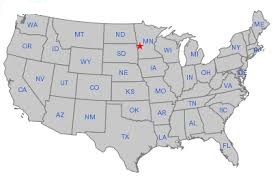
\includegraphics[scale=0.7]{morris.jpg}
\end{figure}
%{\tt Need a map here; need to make bullet points appear one by one}
\begin{itemize}
\item Morris: rural town 3.5 hours from UMN-TC. 
\item UMM:  small undergraduate-only liberal arts college.
\item Undergraduate research. 
\item<2>Use Lisp in an introductory CS class. 
\end{itemize}
\end{frame}

\begin{frame}
   \frametitle{A programming language for introductory class}
\begin{itemize}
\item {\bf Use} a programming language in an introductory class.
\item {\bf  Teach} concepts and skills.
\item {\bf  Teach} CS-style problem solving.
\item The language needs to be simple, well-defined, and non-distracting (Felleisen et al, 2004).
\item Dynamically typed.
\item Functional languages are useful: focus on functions, modularity, abstraction.
\item Functional languages: higher order functions (needed now with Javascript-based web dev)
\item Interactive development: REPL. 
%\item Lisps have simple syntax and clearly defined semantics.
\end{itemize}
\end{frame}

\begin{frame}
   \frametitle{Current use of Lisp/Clojure in classes}
\begin{itemize}
\item UMM uses Racket (a Lisp) in an introductory class. 
\item 2010: a UMM student mentioned Clojure. 
\item We've used Clojure in upper-level courses (Programming Languages, Programming for Parallel Architecture).
\item Would like to use it in an introductory class (it's a long way).
\item A couple of other schools use Clojure: Hampshire College, MA. 
\end{itemize}
\end{frame}

\begin{frame}
   \frametitle{What Clojure brings to the table?}
Students are curious, would like to expand and apply what they learn. 

Clojure offers:
\begin{itemize}
\item A large community that students can explore/benefit from: libraries, community-maintained docs, textbooks, blog posts, open source projects, meetups,....
\item Concurrency.
\item Integration with Java. 
\end{itemize}
\end{frame}

\section{Why {\bf not} (yet) Clojure}

\begin{frame}
   \frametitle{What's lacking}
\begin{itemize}
\item Usability of error messages. {\tt give an example}
\item Beginner-friendly IDE. 
\item Beginner-friendly project manager. 
%\item Can't expect new students use emacs/vim and command line (at least if we want to keep CS enrollments/diversity). 
\item Beginner-friendly graphical libraries. 
\item More uniform behavior of strings, collections vs sequences, etc.   {\tt give an example}
\item Beginner-friendly textbooks (focus on concepts, use language as a learning tool). 
\end{itemize}
\end{frame}

\section{Error messages transformations}
\begin{frame}
   \frametitle{(Non)Usability of error messages}
 {\tt give an example -- perhaps better to just give an example?}
\begin{itemize}
\item Phrased in terms of Java types.
\item Java stack trace. 
\item Often misleading. 
\item Not particularly well integrated with IDEs (LightTable does some line highlighting). 
\item Come from compiler, run-time system, REPL, testing frameworks (makes integration with IDE difficult). 
\end{itemize}
\end{frame}

\begin{frame}
   \frametitle { What do we do about error messages}
\begin{itemize}
\item {\tt Post-processing Clojure messages}. 
\item Filter stack trace.
\item Transform using regular expressions. 
\item Add pre-conditions to common functions ({\tt map, filter,} etc). 
\end{itemize}
\end{frame}

\subsection{Regular expressions}

\subsection{Pre-conditions}
\begin{frame}[fragile]
   \frametitle {Adding pre-conditions to common functions }
Student code:
\begin{verbatim}
(map "inc" [1 2 3])
\end{verbatim} 

Original error message:
\begin{verbatim}
ClassCastException java.lang.String cannot be cast to
clojure.lang.IFn  clojure.core/map/fn--4245 (core.clj:257)
\end{verbatim} 

Our error message: 
\begin{verbatim}
In function map, the first argument "inc" must be
a function but is a string.
\end{verbatim}
\end{frame}

\begin{frame}
 \frametitle {Benefits and issues}
\begin{itemize}
\item Can determine specific arguments that caused an error. 
\item Need to overwrite many functions (e.g. arithmetic functions).
\item 
\item We overwrite predefined functions: need to load them into student code. 
\end{itemize}
\end{frame}

\subsection{Idea: hints and scenarios}

\section{Beginner-friendly tools}

\begin{frame}
   \frametitle{Error messages processing}
\begin{itemize}
\item Minimal interference with IDE or leiningen.
\item Need to catch error messages from compiler,  run-time system, REPL, testing.
\item Looked into: integrating with IDE (LightTable), leiningen plugin. 
\item Current plan for catching error messages: {\tt nrepl} middleware. 
\end{itemize}
\end{frame}

\begin{frame}
   \frametitle{Leiningen plugin}
\begin{itemize}
\item Need to load functions with pre-conditions (and perhaps more) into student code. 
\item 
\item 
\end{itemize}
\end{frame}

\section{Future work (lots of it!), acknowledgments}

\begin{frame}
   \frametitle{Future work}
\begin{itemize}
\item 
\item Usability studies. 
\item 
\end{itemize}
\end{frame}

\begin{frame}
   \frametitle{Many thanks to:}
\begin{itemize}
\item UMM students who started this project: Brian Goslinga, Stephen Adams, Joe Einertson. 
\item UMM students who worked on it in 2013/15: Max Magnuson, Paul Schliep, Henry Fellows, Emma Sax, Aaron Lemmon. 
\item My colleagues and friends: Jon Anthony, Michael Bukatin, Simon Hawkin, Nic McPhee. 
\item MN Clojure group and Boston Clojure meetup. 
\end{itemize}
\end{frame}

\begin{frame}
   \frametitle{Our resources}
\begin{itemize}
\item 
\end{itemize}
\end{frame}

\end{document}
